\documentclass[main.tex]{subfiles}
\begin{document}
\chapter{Decrease and Conquer}
Want to do even better than  linear complexity? Decrease and conquer reduces one problem into one smaller subproblem only, and the most common case is to reduce the state space into half of its original size. If the combining step takes only constant time, we get an elegant recurrence relation as:
\begin{equation}
    T(n) = T(n/2) + O(1),
\end{equation}
which gives us logarithmic time complexity!

We introduce three classical algorithms--binary search in array, binary search tree, and segment tree to enforce our understanding of decrease and conquer. Importantly, binary search and binary search tree consists \textbf{10\%} of the total interview questions. 
\section{Introduction}
All the searching we have discussed before never assumed any ordering between the items, and searching an item in an unordered space is doomed to have a time complexity linear to the space size. This case is about to change in this chapter. 

Think about these two questions: What if we have a sorted list instead of an arbitrary one? What if the parent and children nodes within a tree are ordered in some way? With such special ordering between items in a data structures, can we increase its searching efficiency and be better than the blind one by one search in the state space? The answer is YES.

Let's take advantage of the ordering and the decrease and conquer methodology. To find a target in a space of size $n$, we first divide it into two subspaces and each of size $n/2$, say from the middle of the array. If the array is increasingly ordered, all items in the left subspace are smaller than all items in the right subspace. If we compare our target with the item in the middle, we will know if this target is on the left or right side. With just one step, we reduced our state space by half size. We further repeat this process on the reduced space until we find the target. This process is called \textbf{Binary Search}. Binary search has recurrence relation:
\begin{equation}
   T(n) = T(n/2) + O(1) ,
\end{equation}
which decreases the time complexity from $O(n)$ to $O(\log n)$.

  
%%%%%%%%%Binary search%%%%%%%%%
\section{Binary Search}
Binary search can be easily applied in sorted array or string. 
\begin{lstlisting}[numbers=none]
For example, given a sorted and distinct array
nums = [1, 3, 4, 6, 7, 8, 10, 13, 14, 18, 19, 21, 24, 37, 40, 45, 71]
Find target t = 7.
\end{lstlisting}
\paragraph{Find the Exact Target}
\begin{figure}[H]
    \centering
    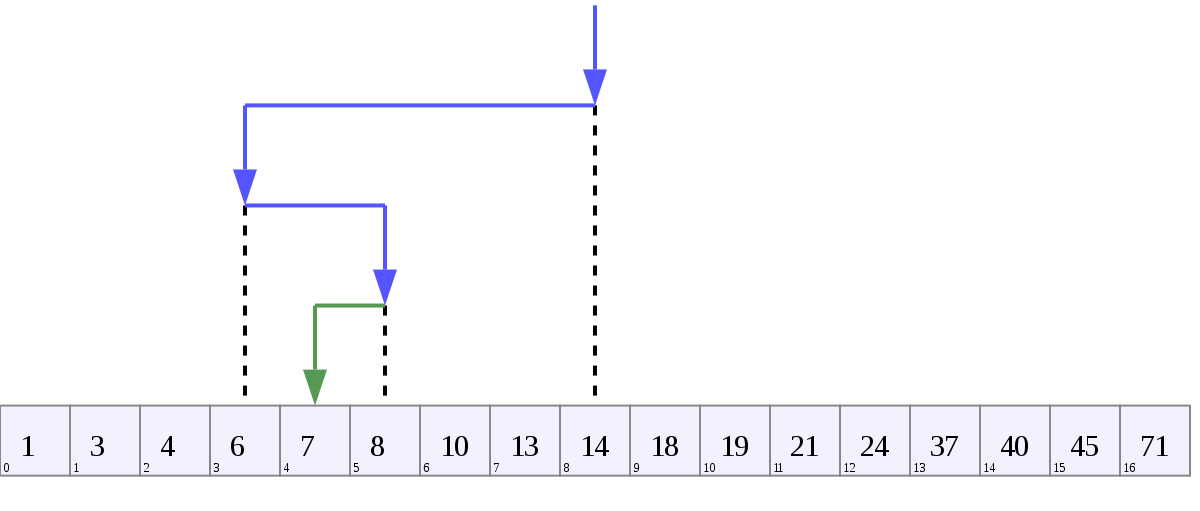
\includegraphics[width=0.7\columnwidth]{fig/Binary_Search_Depiction.png}
    \caption{Example of Binary Search}
    \label{fig:binary_search_eg_1}
\end{figure}

This is the most basic application of binary search. We can set two pointers, \texttt{l} and \texttt{r}, which points to the first and last position, respectively. Each time we compute the middle position \texttt{m = (l+r)//2}, and check if the item $num[m]$ is equal to the target \texttt{t}. 
\begin{itemize}
\item If it equals, target found and return the position. 
\item If it is smaller than the target, move to the left half by setting the right pointer to the position right before the middle position, $r = m - 1$. 
\item If it is larger than the target, move to the right half by setting the left pointer to the position right after the middle position, $l = m + 1$. 
\end{itemize}
Repeat the process until we find the target or we have searched the whole space. The criterion of finishing the whole space is when \texttt{l} starts to be larger than $r$. Therefore, in the implementation we use a \texttt{while} loop with condition \texttt{l$\leq$ r} to make sure we only scan once of the searching space. The process of applying binary search on our exemplary array is depicted in Fig.~\ref{fig:binary_search_eg_1} and the Python code is given as:
\begin{lstlisting}[language=Python]
def standard_binary_search(lst, target):
    l, r = 0, len(lst) - 1
    while l <= r:
        mid = l + (r - l) // 2
        if lst[mid] == target:
            return mid
        elif lst[mid] < target:
            l = mid + 1
        else:
            r = mid - 1
    return -1 # target is not found 
\end{lstlisting}
In the code, we compute the middle position with \texttt{mid = l + (r - l) // 2} instead of just \texttt{mid = (l + r) //2} because these two always give the same computational result but the later is more likely to lead to overflow with its addition operator.

\subsection{Lower Bound and Upper Bound}
\paragraph{Duplicates and Target Missing} What if there are duplicates in the array:
\begin{lstlisting}[numbers=none]
For example, 
nums = [1, 3, 4, 4, 4, 4, 6, 7, 8]
Find target t = 4
\end{lstlisting}
Applying the first standard binary search will return \texttt{3} as the target position, which is the second $4$ in the array. This does not seem like a problem at first. However, what if you want to know the predecessor or successor (3 or 5) of this target? In a distinct array, the predecessor and successor would be adjacent to the target. However, when the target has duplicates, the predecessor is  before the first target and the successor is next to the last target. Therefore, returning an arbitrary one will not be helpful. 

Another case, what if our target is 6, and we first want to see if it exists in the array. If it does not, we would like to insert it into the array and still keep the array sorted. The above implementation simply returns $-1$, which is not helpful at all. 

The \textbf{lower and upper bound} of a binary search are the lowest and highest position where the value could be inserted without breaking the ordering. 
% However, if we design our algorithm to find (1) find the first position that has value larger or equals to the target, and (2) find the last position that has value smaller or equals to the target. This might be bit confusing, let us see it through examples. 

\begin{figure}[H]
    \centering
    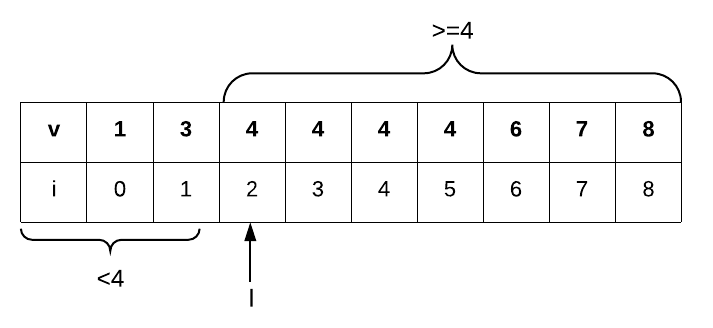
\includegraphics[width=0.9\columnwidth, height=4cm]{fig/binary_search_lower_bound.png}
        \caption{Binary Search: Lower  Bound of target 4.}
            \label{fig:binary_search_eg_lower_bound}
    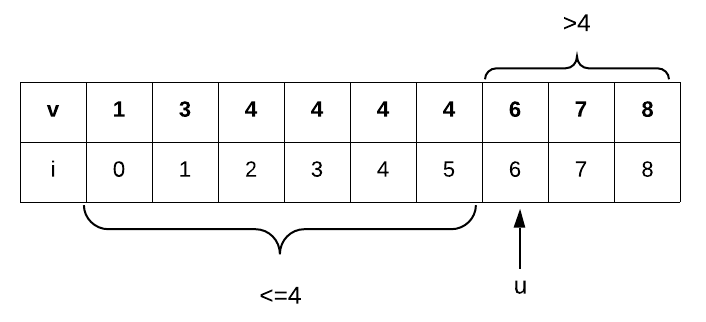
\includegraphics[width=0.9\columnwidth, height=4cm]{fig/binary_search_upper_bound.png}
    \caption{Binary Search: Upper Bound of target 4.}
    \label{fig:binary_search_eg_upper_bound}
\end{figure} 
For example, if our $t=4$, the first position it can insert is at index 2 and the last position is at index 6.
\begin{itemize}
    \item 
With index 2 as the lower bound, 
items in $i \in [0, l-1], a[i]<t$, $a[l] = t$, and $i\in[l, n), a[i] \geq t$. A lower bound is also the first position that has a value \texttt{v $\geq$ t}.  This case is shown in Fig.~\ref{fig:binary_search_eg_lower_bound}.
\item With the upper bound, items in $i \in [0, u-1], a[i]\leq t$, $a[u] = t$, and $i\in[u, n), a[i] > t$. An upper bound is also the first position that has a value \texttt{v > t}.  This case is shown in Fig.~\ref{fig:binary_search_eg_upper_bound}.
\end{itemize}
\begin{figure}[H]
    \centering
    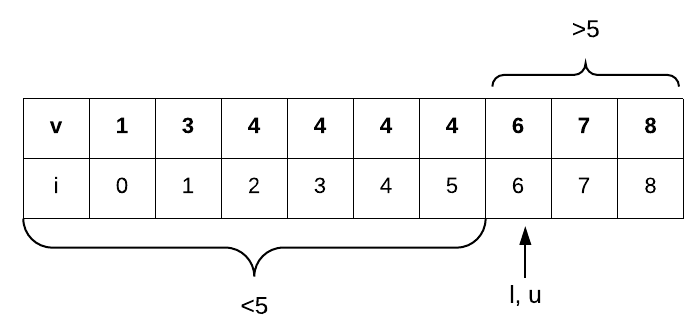
\includegraphics[width=0.9\columnwidth, height=4cm]{fig/binary_search_lower_upper.png}
        \caption{Binary Search: Lower and Upper  Bound of target 5 is the same.}
   
    \label{fig:binary_search_lower_upper}
\end{figure} 


If $t=5$, the only position it can insert is at index 6, which indicates $l = u$. We show this case in Fig.~\ref{fig:binary_search_lower_upper}.

Now that we know the meaning of the upper and lower bound, here comes to the question, ``How to implement them?''

\paragraph{Implement Lower Bound} Because if the target equals to the value at the middle index, we have to move to the left half to find its leftmost position of the same value. Therefore, the logic is that we move as left as possible until it can't  further. When it stops,  $l>r$, and \texttt{l} points to the first position that the value $v$ be $v\geq t$. Another way to think about the return value is with assumption: Assume the middle pointer $m$ is at the first position that equals to the target in the case of target 4, which is index 2. According to the searching rule, it goes to the left search space and changes the right pointer as  $r=m-1$. At this point, in the valid search space, there will never be a value that can be larger or equals to the target, pointing out that it will only moving to the right side, increasing the \texttt{l} pointer and leave the \texttt{r} pointer untouched until  $l > r$ and the search stops. When the first time that $l > r$, the left pointer will be $l = r + 1 = m$, which is the first position that its value equals to the target. 

The search process for target 4 and 5 is described as follows:
\begin{lstlisting}[numbers=none]
0:  l = 0, r = 8, mid = 4
1:  mid = 4, 4==4, l = 0, r = 3
2:  mid = 1, 4>3, l = 2, r = 3
3:  mid = 2, 4==4, l = 2, r = 1
return l=2
\end{lstlisting}
Similarly, we run the case for target 5. 
\begin{lstlisting}[numbers=none]
0:  l = 0, r = 8, mid = 4
1:  mid = 4, 5>4, l = 5, r = 8
2:  mid = 6, 5<6, l = 5, r = 5
3:  mid = 5, 5>4, l = 6, r = 5
return l=6
\end{lstlisting}
The Python code is as follows:
\begin{lstlisting}[language=Python]
def lower_bound_bs(nums, t):
  l, r = 0, len(nums) - 1
  while l <= r:
    mid = l + (r - l) // 2
    if t <= nums[mid]: # move as left as possible
      r = mid - 1
    else:
      l = mid + 1
  return l
\end{lstlisting}
\paragraph{Implement Upper Bound} To be able to find the upper bound, we need to move the left pointer to the right as much as possible. Assume we have the middle index at 5, with target as 4. The binary search moves  to the right side of the state space, making $l=mid+1=6$. Now, in the right state space, the middle pointer will always have values larger than 4, thus it will only moves to the left side of the space, which only changes the right pointer \texttt{r} and leaves the left pointer \texttt{l} touched when the program ends. Therefore, \texttt{l} will still return our final upper bound index.  The Python code is as follows:
\begin{lstlisting}[language=Python]
def upper_bound_bs(nums, t):
  l, r = 0, len(nums) - 1
  while l <= r:
    mid = l + (r - l) // 2
    if t >= nums[mid]: # move as right as possible
      l = mid + 1
    else:
      r = mid - 1
  return l
\end{lstlisting}


\paragraph{Python Module \texttt{bisect}}
% Binary search is usually carried out on a Static sorted array or 2D matrix. There are three basic cases: (1) find the exact target that value = target; If there are duplicates, we are more likely to be asked to (2) find the first position that has value >= target; (3) find the first position that has value <= target. Here, we use two example array: one without duplicates and the other has duplicates.
% \begin{lstlisting}[language=Python]
% a = [2, 4, 5, 9]
% b = [0, 1, 1, 1, 1, 1]
% \end{lstlisting}


% From the example, we can see that multiple \textbf{duplicates} of the target exist, it can possibly return any one of them. And for the case when the target does not exist, it simply returns -1. In reality, we might need to find a position where we can potentially insert the target to keep the sorted array sorted. There are two cases: (1) the first position that we can insert, which is the first position that has value>= target (2) and the last position we can insert, which is the first position that has value > target. For example, if we try to insert 3 in a, and 1 in b, the first position should be 1 and 1 in each array, and the last position is 1 and 6 instead.  
Conveniently, we have a Python built-in Module \texttt{bisect} that offers two methods: \texttt{bisect\_left()} for obtaining the lower bound and \texttt{bisect\_right()} to obtain the upper bound. For example, we can use it as:
\begin{lstlisting}[language=Python]
from bisect import bisect_left,bisect_right, bisect
l1 = bisect_left(nums, 4)
r1 = bisect_right(nums, 5)
l2 = bisect_right(nums, 4)
r2 = bisect_right(nums, 5)
\end{lstlisting}
It offers six methods as shown in Table~\ref{tab:method_bisect}. 
\begin{table}[h]
\begin{small}
\centering
\noindent\captionof{table}{ Methods of \textbf{bisect}}
 \noindent \begin{tabular}{|p{0.25\columnwidth}|p{0.75\columnwidth}| }
  \hline
Method & Description   \\ \hline
\texttt{bisect\_left(a, x, lo=0, hi=len(a)}  &  The parameters lo and hi may be used to specify a subset of the list; the function is the same as bisect\_left\_raw  \\\hline
\texttt{bisect\_right(a, x, lo=0, hi=len(a)}  &  The parameters lo and hi may be used to specify a subset of the list; the function is the same as bisect\_right\_raw  \\\hline
\texttt{bisect(a, x, lo=0, hi=len(a))}  &Similar to bisect\_left(), but returns an insertion point which comes after (to the right of) any existing entries of x in a.\\ \hline
\texttt{insort\_left(a, x, lo=0, hi=len(a))}  &This is equivalent to a.insert(bisect.bisect\_left(a, x, lo, hi), x).\\ \hline
\texttt{insort\_right(a, x, lo=0, hi=len(a))} & This is equivalent to a.insert(bisect.bisect\_right(a, x, lo, hi), x).\\ \hline
\texttt{insort(a, x, lo=0, hi=len(a))} & Similar to insort\_left(), but inserting x in a after any existing entries of x.\\ \hline
\end{tabular}
  \label{tab:method_bisect}
  \end{small}
\end{table} 

\paragraph{Bonus} For the lower bound, if we return the position as l-1, then we get the last position that \texttt{value < target}. Similarily, for the upper bound, we get  the last position \texttt{value <= target}.

% \paragraph{Python Built-in Module bisect} This module provides support for maintaining a list in sorted order without having to sort the list after each insertion. I
% Let's see come examplary code:
% \begin{lstlisting}[language=Python]
% from bisect import bisect_left,bisect_right, bisect
% print("bisect left: find 3 in a :", bisect_left(a,3), 'find 1 in b: ', bisect_left(b, 1)) # lower_bound, the first position that value>= target
% print("bisect right: find 3 in a :", bisect_right(a, 3), 'find 1 in b: ', bisect_right(b, 1)) # upper_bound, the last position that value <= target
% \end{lstlisting}
% The print out is:
% \begin{lstlisting}
% bisect left: find 3 in a : 1 find 1 in b:  1
% bisect right: find 3 in a : 1 find 1 in b:  6
% \end{lstlisting}
\subsection{Applications}
\label{concept_binary_search_in_array}
Binary Search is a powerful problem solving tool. Let's go beyond the sorted array: How about when the array is sorted in a way that  is not as monotonic as what we are familiar with, or how about solving math functions with binary search, whether they are continuous or discrete, equations or inequations?
\paragraph{First Bad Version(L278)} You are a product manager and currently leading a team to develop a new product. Unfortunately, the latest version of your product fails the quality check. Since each version is developed based on the previous version, all the versions after a bad version are also bad.

Suppose you have $n$ versions [1, 2, ..., n] and you want to find out the first bad one, which causes all the following ones to be bad. You are given an API \texttt{bool isBadVersion(version)} which will return whether version is bad. Implement a function to find the first bad version. You should minimize the number of calls to the API.
\begin{lstlisting}[numbers=none]
Given n = 5, and version = 4 is the first bad version.

call isBadVersion(3) -> false
call isBadVersion(5) -> true
call isBadVersion(4) -> true

Then 4 is the first bad version.
\end{lstlisting}
\paragraph{Analysis and Design} In this case, we have a search space in range $[1, n]$. Think the value at each position is the result from function \texttt{isBadVersion(i)}. Assume the first bad version is at position $b$, then the values from the positions are of such pattern: [F,..., F, ..., F, T, ..., T]. We can totally apply the binary search in the search space $[1, n]$: to find the first bad version is the same as finding the first position that we can insert a value \texttt{True}--the lower bound of value \texttt{True}. Therefore, whenever the value we find is \texttt{True}, we move to the left space to try to get its first location. The Python code is given below:
\begin{lstlisting}[language = Python]
def firstBadVersion(n):
    l, r = 1, n
    while l <= r:
        mid = l + (r - l) // 2
        if isBadVersion(mid):
            r = mid - 1
        else:
            l = mid + 1           
    return l
\end{lstlisting}
\subsubsection{Search in Rotated Sorted Array}
``How about we rotate the sorted array?''
\paragraph{Problem Definition(L33, medium)} Suppose an array (without duplicates) is first sorted in ascending order, but later is rotated at some pivot unknown to you beforehand--it takes all items before the pivot to the end of the array. For example, an array [0, 1, 2, 4, 5, 6, 7] be rotated at pivot 4, will become [4, 5, 6, 7, 0, 1, 2]. If the pivot is at 0, nothing will be changed. If it is at the end of the array, say 7, it becomes [7, 0, 1, 2, 4, 5, 6]. You are given a target value to search. If found in the array return its index, otherwise return -1. 
\begin{lstlisting}[numbers=none]
Example 1:
Input: nums = [3,4,5,6,7,0,1,2], target = 0
Output: 5

target = 8
Output: -1
\end{lstlisting}
\paragraph{Analysis and Design}
In the rotated sorted array, the array is not purely monotonic. Instead, there will be at most  one drop in the array because of the rotation, which we denote the high and the low item as $a_h, a_l$ respectively. This drop  cuts the array into two parts: $a[0:h+1]$ and $a[l:n]$, and both parts are ascending sorted. If the middle point falls within the left part, the left side of the state space will be sorted, and if it falls within the right part, the right side of the state space will be sorted.  Therefore, at any situation, there will always be one side of the state space that is sorted. To check which side is sorted, simply compare the value of middle pointer with that of left pointer. 
\begin{itemize}
    \item If \texttt{nums[l] < nums[mid]}, then the left part is sorted.
    \item If \texttt{nums[l] > nums[mid]}, then the right part is sorted.
    \item Otherwise when they equal to each other, which is only possible that there is no left part left, we have to move to the right part. For example, when \texttt{nums=[1, 3]}, we move to the right part.
\end{itemize}

With a sorted half of state space, we can check if our target is within the sorted half: if it is, we switch the state space to the sorted space; otherwise, we have to move to the other half that is unknown. The Python code is shown as:
\begin{lstlisting}[language=Python]
def RotatedBinarySearch(nums, t):   
      l, r = 0, len(nums)-1
      while l <= r:
          mid = l + (r-l)//2
          if nums[mid] == t:
              return mid
          # Left is sorted
          if nums[l] < nums[mid]: 
              if nums[l] <= t < nums[mid]:
                  r = mid - 1
              else:
                  l = mid + 1
          # Right is sorted
          elif nums[l] > nums[mid]: 
              if nums[mid] < t <= nums[r]:
                  l = mid + 1
              else:
                  r = mid - 1
          # Left and middle index is the same, move to the right
          else: 
              l = mid + 1
      return -1
\end{lstlisting}
\begin{bclogo}[couleur = blue!30, arrondi=0.1,logo=\bccrayon,ombre=true]{What happens if there are duplicates in the rotated sorted array? } In fact, the same comparison rule applies, with one minor change. When \texttt{nums=[1, 3, 1, 1, 1]}, the middle pointer and the left pointer has the same value, and in this case, the right side will only consist of a single value, making us to move to the left side instead. However, if \texttt{nums=[1,1,3]}, we need to move to the right side instead.  Moreover, for \texttt{nums=[1, 3]}, it is because there is no left side we have to search the the right side. Therefore, in this case, it is impossible for us to decide which way to go, a simple strategy is to just move the left pointer forward by one position and retreat to the linear search. 
\begin{lstlisting}[language=Python]
# The left half is sorted
if nums[mid] > nums[l]: 
# The right half is sorted
elif nums[mid] < nums[l]: 
# For third case
else: 
   l +=1 
\end{lstlisting}
\end{bclogo}




%%%%%%%%%%%%%%binary search on result space%%%%%%%
\subsubsection{Binary Search to Solve Functions}
Now, let's see how it can be applied to solve equations or inequations. Assume, our function is $y = f(x)$, and this function is monotonic, such as $y = x, y = x^2+1, y = \sqrt{x}$. To solve this function is the same as finding a solution $x_t$ to a given target $y_t$. We generally have three steps to solve such problems: % If the question gives us the context: the target is in the range [left, right], we need to search the first or last position that satisfy a condition function. We can apply the concept of standard binary search and bisect\_left and bisect\_right and its mutant. Where we use the condition function to replace the value comparison between target and element at middle position. The steps we need:
\begin{enumerate}
    \item Set a search space for $x$, say it is $[x_l, x_r]$. 
    \item If the function is equation, we find a $x_t$ that either equals to $y_t$ or close enough such as $|y_t - y| <= 1e-6$ using standard binary search. 
    \item If the function is inequation, we see if it wants the first or the last $x_t$ that satisfy the constraints on $y$. It is the same as of finding the lower bound or upper bound. 
\end{enumerate}

\paragraph{Arranging Coins (L441, easy)} You have a total of n coins that you want to form in a staircase shape, where every $k$-th row must have exactly $k$ coins. Given n, find the total number of full staircase rows that can be formed. n is a non-negative integer and fits within the range of a 32-bit signed integer.
\begin{lstlisting}[numbers=none]
Example 1:
n = 5
The coins can form the following rows:
*
* *
* *

Because the 3rd row is incomplete, we return 2.
\end{lstlisting}

\paragraph{Analysis and Design} Each row $x$ has $x$ coins, summing it up, we get $1+2+...+x= \frac{x(x+1)}{2}$. The problem is equvalent to find the last integer $x$ that makes $\frac{x(x+1)}{2}\leq n$. Of course, this is just a quadratic equation which can be easily solved if you remember the formula, such as the following Python code:
\begin{lstlisting}[language=Python]
import math
def arrangeCoins(n: int) -> int:
    return int((math.sqrt(1+8*n)-1) // 2)
\end{lstlisting}
However, if in the case where we do not know a direct closed-form solution, we solicit binary search. First, the function of $x$ is monotonically increasing, which indicates that binary search applies. We set the range of $x$ to $[1, n]$, what we need is to find the last position that the condition of  $\frac{x(x+1)}{2}\leq n$ satisfies, which is the position right before the upper bound. The Python code is given as:
\begin{lstlisting}[language=Python]
def arrangeCoins(n):
    def isValid(row):
        return (row * (row + 1)) // 2 <= n
    
    def bisect_right():
        l, r = 1, n
        while l <= r:
            mid = l + (r-l) // 2
            # Move as right as possible
            if isValid(mid): 
                l = mid + 1
            else:
                r = mid - 1
        return l
    return bisect_right() - 1
\end{lstlisting}

% \subsection{Bisection Method} (second edition)
% The binary search principle can be used to find the root of a function that may be difficult to compute mathematically. We have not seen any problems that require this method on LeetCode yet. Thus we define the problem as:

% Find the monthly payment for a loan: You want to buy a car using loan and want to pay in monthly installment of d d
% \subsection{Python Library}
% Python has \textbf{bisect} module for binary search. 
% \begin{lstlisting}[numbers=none]
% bisect.bisect_left(a,    x):  Return the leftmost index where we can  insert x into a to maintain sorted order! Leftmost rl that satisfy: x<=a[rl]

% bisect.bisect_right(a,    x):  Return the rightmost index where we can  insert x into a to maintain sorted order! Right most rr that satisfy: x>=a[rr]
% \end{lstlisting}
% For example:
% \begin{lstlisting}[language=Python]
% from bisect import bisect_left,bisect_right
% a = [1,    2,    3,    3,    3,    4,    5]
% p1, p2= bisect_left(a,3), bisect_right(a, 3)
% print(p1, p2)
% # output
% # 2, 5
% \end{lstlisting}


%%%%%%%%%%%%%%%%%%%%%binary search tree%%%%%%%%%%%%%%%%%%%%%%
\section{Binary Search Tree}
\label{sec_binary_search_tree}

A sorted array supports logarithmic query time with binary search, however it still takes linear time to update--delete or insert items. Binary search tree (BSTs), a type of binary tree designed for fast access and updates to items,  on the other hand, only takes $O(\log n)$ time to update. How does it work?

In the array data structure, we simply sort the items, but how to apply sorting in a binary tree?  Review the min-heap data structure, which recursively defining a node to have the largest value among the nodes that belong to the subtree of that node, will give us a clue. In the binary search tree, we define that for any given node \texttt{x}, all nodes in the left subtree of \texttt{x} have keys smaller than \texttt{x} while all nodes in the right subtree of \texttt{x} have keys larger than \texttt{x}. An example is shown in Fig.~\ref{fig:bst}. With this definition, simply comparing a search target with the root can point us to half of the search space, given the tree is balanced enough. Moreover, if we do in-order traversal of nodes in the tree from the root, we end up with a nice and sorted keys in ascending order, making binary search tree one member of the sorting algorithms. 
\begin{figure}[H]
    \centering
    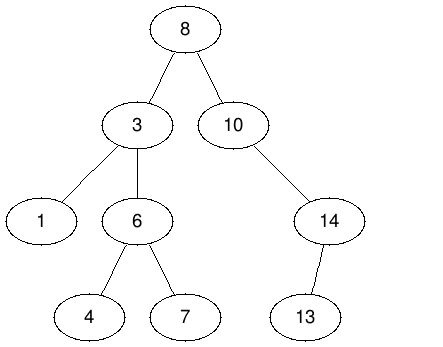
\includegraphics[width = 0.6\columnwidth]{fig/bst_example.png}
    \caption{Example of Binary search tree of depth 3 and 8 nodes.}
    \label{fig:bst}
\end{figure}




% The advantage of search trees is their efficient search time ( $O(\log n)$) given the tree is reasonably balanced, which is to say the leaves at either end are of comparable depths as we introduced the \textbf{balanced binary tree}. 
Binary search tree needs to support many operations, including searching for a given key, the minimum and maximum key, and a  predecessor or successor of a given key, inserting and deleting items while maintaining the binary search tree property. Because of its efficiency of these operations compared with other data structures,  binary search tree is often used as a dictionary or a priority queue.


% Search trees are often used to implement an associative array. The search tree algorithm uses the key from the key-value pair to find a location, and then the application stores the entire key–value pair at that location. 

% In this section, we will introduce the most commonly used two types of searching trees: binary searching tree (BST) and Trie where the keys are usually numeric numbers and strings respectively. 

% \subsection{Binary Searching Tree}
% \label{concept_binary_search_tree}
With $l$ and $r$ to represent the left and right child of node $x$,  there are two other definitions other than the binary search tree definition we just introduced:  (1)$l.key \leq x.key < r.key$ and (2) $l.key  < x.key \leq r.key$. In these two cases, our resulting BSTs allows us to have duplicates. The exemplary implementation follow the definition that does not allow duplicates.

% an organized searching tree structure in binary tree, as the name suggests. Binary search trees whose internal nodes each store a key (and optionally, an associated value), each node have two distinguished sub-trees (if only one sub-tree the other is None). 

% BST keep their keys in sorted order, so that lookup and other operations can use the \textit{principle of binary search tree}: 

% \indent Let $x$ be a node in a binary search tree, if $y$ is a node in the left subtree of x, them $y.key \leq x.key$. If $y$ is a node in the right subtree of $x$, then $y.key \geq x.key$. 



\subsection{Operations}
% When looking for a key in a tree (or a place to insert a new key), we traverse the tree from root to leaf, making comparisons to keys stored in the nodes of the tree and deciding, on the basis of the comparison, to continue searching in the left or right subtrees. On average, this means that each comparison allows the operations to skip about half of the tree, so that each SEARCH, INSERT or DELETE takes time proportional to the logarithm of the number of items stored in the tree. This is much better than the linear time required to find items by key in an (unsorted) array, but slower than the corresponding operations on hash tables. 

% \textbf{Definition} A binary search tree is a rooted binary tree, whose internal nodes each store a key (and optionally, an associated value) and each have two distinguished sub-trees, commonly denoted left and right. The tree additionally satisfies the binary search property, which states that the key in each node must be greater than or equal to any key stored in the left sub-tree, and less than or equal to any key stored in the right sub-tree.[1]:287 The leaves (final nodes) of the tree contain no key and have no structure to distinguish them from one another. 

In order to build a BST, we need to insert a series of items in the tree organized by the search tree property. And in order to insert, we need to search for a proper position first and then insert the new item while sustaining the search tree property. Thus, we introduce these operations in the order of search, insert and generate. 

\paragraph{Search}

The search is highly similar to the binary search in the array. It starts from the root. Unless the node's value equals to the target, the search proceeds to either the left or right child depending upon the comparison result. The search process terminates when either the target is found or when an empty node is reached. It can be implemented either recursively or iteratively with a time complexity $O(h)$, where $h$ is the height of the tree, which is roughly $\log n$ is the tree is balanced enough. The recursive search is shown as:
\begin{lstlisting}[language = Python]
def search(root, t):
  if not root:
    return None
  if root.val == t:
    return root
  elif t < root.val:
    return search(root.left, t)
  else:
    return search(root.right, t)
\end{lstlisting}
Because this is a tail recursion, it can easily be converted to iteration,  which helps us save the heap space. The iterative code is given as:
\begin{lstlisting}[language = Python]
# iterative searching
def iterative_search(root,key):
    while root is not None and root.val != key:
        if root.val < key:
            root = root.right
        else:
            root = root.left
    return root
\end{lstlisting}

\begin{bclogo}[couleur = blue!30, arrondi=0.1,logo=\bccrayon,ombre=true]{Write code to find the minimum and maximum key in the BST. } The minimum key locates at the leftmost of the BST, while the maximum key locates at the rightmost of the tree. 
\end{bclogo}

%%%%%%%%%%%%Insertion%%%%%%%%%%%%%%%%%%%%%%
\paragraph{Insert}
\begin{figure}[H]
    \centering
    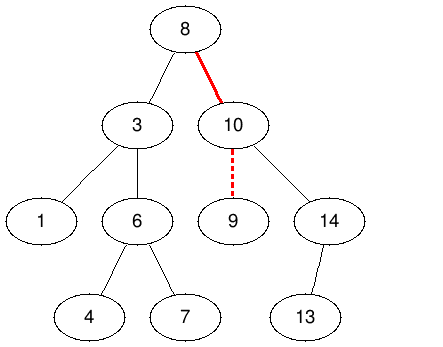
\includegraphics[width=0.6\columnwidth]{fig/bst_insert_9.png}
    \caption{The red colored path  from the root down to the position where the key 9 is inserted. The dashed line indicates the link in the tree that is added to insert the item. }
    \label{fig:bst_insert}
\end{figure}
Assuming we are inserting a node with key 9 into the tree shown in Fig~\ref{fig:bst}. We start from the root, compare 9 with 8, and goes to node 10. Next, the search process will lead us to the left child of node 10, and this is where we should put node 9. The process is shown in Fig.~\ref{fig:bst_insert}. 

The process itself is easy and clean. Here comes to the implementation. We treat each node as a subtree: whenever the search goes into that node, then the algorithm hands over the insertion task totally to that node, and assume it has inserted the new node and return its updated node. The main program will just simply reset its left or right child with the return value from its children. The insertion of new node happens when the search hits an empty node, it returns a new node with the target value. The implementation is given as:
\begin{lstlisting}[language = Python]
def insert(root, t):
  if not root:
    return BiNode(t)
  if root.val == t:
    return root
  elif t < root.val:
    root.left = insert(root.left, t)
    return root
  else:
    root.right = insert(root.right, t) 
    return root
\end{lstlisting}
In the notebook, I offered a variant of implementation, check it out if you are interested. To insert iteratively, we need to track the parent node while searching. The \texttt{while} loop stops when it hit at an empty node.  There will be three cases in the case of the parent node:
\begin{enumerate}
    \item When the parent node is \texttt{None}, which means the tree is empty. We assign the root node with the a new node of the target value.
\item When the target's value is larger than the parent node's, the put a new node as the right child of the parent node.  
\item When the target's value is smaller than the parent node's, the put a new node as the left child of the parent node. 
\end{enumerate}
The iterative code is given as:
\begin{lstlisting}[language = Python]
def insertItr(root, t):
  p = None
  node = root #Keep the root node
  while node:
    # Node exists already
    if node.val == t:
      return root
    if t > node.val:
      p = node
      node = node.right
    else:
      p = node
      node = node.left
  # Assign new node
  if not p:
    root = BiNode(t)
  elif t > p.val:
    p.right = BiNode(t)
  else:
    p.left = BiNode(t)
  return root
\end{lstlisting}
\paragraph{BST Generation}
To generate our exemplary BST shown in Fig.~\ref{fig:bst}, we set \texttt{keys = [8, 3, 10, 1, 6, 14, 4, 7, 13]}, then we call \texttt{insert} function we implemented for each key to generate the same tree. The time complexity will be $O(n\log n)$.
\begin{lstlisting}[language=Python]
keys = [8, 3, 10, 1, 6, 14, 4, 7, 13]
root = None
for k in keys:
  root = insert(root, k)
\end{lstlisting}
\paragraph{Find the Minimum and Maximum Key} Because the minimum key is the leftmost node within the tree, the search process will always traverse to the left subtree and return the last non-empty node, which is our minimum node.  The time complexity is the same as of searching any key, which is $O(\log n)$.
\begin{lstlisting}[language=Python]
def minimum(root):
  if not root:
    return None
  if not root.left:
    return root
  return minimum(root.left)
\end{lstlisting}
It can easily be converted to iterative:
\begin{lstlisting}[language=Python]
def minimumIter(root):
  while root:
    if not root.left:
      return root
    root = root.left
  return None
\end{lstlisting}
To find the maximum node, replacing \texttt{left} with \texttt{right} will do. 
%%%%%%%%%%%Predecessor and Successor
Also, sometimes we need to search two additional items related to a given node:  successor and predecessor. The structure of a binary search tree allows us to determine the successor or the predecessor of a tree without ever comparing keys. 

\paragraph{Successor}  A successor of node $x$ is the smallest node in BST that is strictly greater than $x$. It is also called \textbf{in-order successor}, which is the node next to node $x$ in the inorder traversal ordering--sorted ordering. Other than the maximum node in BST, all other nodes will have a successor. The simplest implementation is to return the next node within inorder traversal. This will have a linear time complexity, which is not great. The code is shown as:
\begin{lstlisting}[language=Python]
def successorInorder(root, node):
  if not node:
    return None
  if node.right is not None:
    return minimum(node.right)
  # Inorder traversal
  succ = None
  while root:      
    if node.val > root.val:
      root = root.right
    elif node.val < root.val:
      succ = root
      root = root.left
    else:
      break
  return succ
\end{lstlisting}

Let us try something else. In the BST shown in Fig.~\ref{fig:bst_insert}, the node 3's successor will be node 4. For node 4, its successor will be node 6. For node 7, its successor is node 8. What are the cases here?
\begin{itemize}
    \item An easy case is when a node has right subtree, its successor is the minimum node within its right subtree.
    \item However, if a node does not have a right subtree, there are two more cases: 
    \begin{itemize}
        \item If it is a left child of its parent, such as node 4 and 9, its direct parent is its successor.
        \item However, if it is a right child of its parent, such as node 7 and 14, we traverse backwards to check its parents. If a parent node is the left chid of its parent, then that parent will be the successor. For example, for node 7, we traverse through 6, 3, and 3 is a left child of node 8, making node 8 the successor for node 7.  
    \end{itemize}
    The above two rules can be merged as: starting from the target node, traverse backward to check its parent, find the first two  nodes which are in left child--parent relation. The parent node in that relation will be our targeting successor. Because the left subtree is always smaller than a node, when we backward, if a node is smaller than its parent, it tells us that the current node is smaller than that parent node too. 
\end{itemize}
We write three functions to implement the successor: 
\begin{itemize}
    \item Function \texttt{findNodeAddParent} will find the target node and add a \texttt{parent} node to each node along the searching that points to their parents. The Code is as:
\begin{lstlisting}[language=Python]
def findNodeAddParent(root, t):
  if not root:
    return None
  if t == root.val: 
    return root
  elif t < root.val:
    root.left.p = root
    return findNodeAddParent(root.left, t)
  else:
    root.right.p = root
    return findNodeAddParent(root.right, t)
\end{lstlisting}
\item Function \texttt{reverse} will find the first left-parent relation when traverse backward from a node to its parent.
\begin{lstlisting}[language=Python]
def reverse(node):
  if not node or not node.p:
    return None
  # node is a left child
  if node.val < node.p.val:
    return node.p
  return reverse(node.p)
\end{lstlisting}
\item Function \texttt{successor} takes a node as input, and return its sccessor.
\begin{lstlisting}[language=Python]
def successor(root):
  if not root:
    return None
  if root.right:
    return minimum(root.right)
  else:
    return reverse(root) 
\end{lstlisting}
\end{itemize}
To find a successor for a given key, we use the following code:
\begin{lstlisting}[language=Python]
root.p = None
node = findNodeAddParent(root, 4)
suc = successor(node)
\end{lstlisting}
This approach will gives us $O(\log n)$ time complexity. 
% \parabutbut if is only possible with parent nodes. For BST that has no parent nodes designed, we can add parent nodes along searching the target node. After the target node is found, we stop and check different cases. The code is given as:
% \begin{lstlisting}[language=Python]
% def successor(root, t):
%   # Traverse backward and see if a node is a left child
%   def reverse(node):
%     if not node or not node.p:
%       return None
%     # node is a left child
%     if node.val < node.p.val:
%       return node.p
%     return reverse(node.p)
  
%   # Find the target and set its parent while searching
%   def helper(root, t):
%     # t is not found
%     if not root:
%       return None
%     if t == root.val: 
%       if root.right:
%         return minimum(root.right)
%       else:
%         return reverse(root)
%     elif t < root.val:
%       root.left.p = root
%       return helper(root.left, t)
%     else:
%       root.right.p = root
%       return helper(root.right, t)
    
%   root.p = None
%   return helper(root, t)
% \end{lstlisting}

% Use parent node: the algorihtm has two cases on the basis of the right subtree of the input node. 
% \begin{lstlisting}[numbers=none]
% For the right subtree of the node:
% 1) If it is not None, then the successor is the minimum node in the right subtree. e.g. for node 12, successor(12) = 13 = min(12.right)
% 2) If it is None, then the successor is one of its ancestors. We traverse up using the parent node until we find a node which is the left child of its parent. Then the parent node here is the successor. e.g.  successor(2)=5
% \end{lstlisting}
%  The Python code is provided:
% \begin{lstlisting}[language = Python]
% def Successor(root, n):
% # Step 1 of the above algorithm
%     if n.right is not None:
%         return get_minimum(n.right)
% # Step 2 of the above algorithm
% p = n.parent
% while p is not None:
%     if n == p.left :# if current node is the left child node, then we found the successor, p
%         return p
%     n = p
%     p = p.parent
% return p
% \end{lstlisting}


\paragraph{Predecessor}  A predecessor of node $x$ on the other side, is the largest item in BST that is strictly smaller than $x$. It is also called \textbf{in-order predecessor}, which denotes the previous node in Inorder traversal of BST. For example, for node 6, the predecessor is node 4, which is the maximum node within its left subtree. For node 4, its predecessor is node 3, which is the parent node in a right child--parent relation while tracing back through parents. Now, assume we find the targeting node with function \texttt{findNodeAddParent}, we first write \texttt{reverse} function as \texttt{reverse\_right}. 
\begin{lstlisting}[language=Python]
def reverse_right(node):
  if not node or not node.p:
    return None
  # node is a right child
  if node.val > node.p.val:
    return node.p
  return reverse_right(node.p)
\end{lstlisting}
Next, we implement the above rules to find predecessor of a given node. 
\begin{lstlisting}[language = Python]
def predecessor(root):
  if not root:
    return None
  if root.left:
    return maximum(root.left)
  else:
    return reverse_right(root) 
\end{lstlisting}
 The expected time complexity is $O(\log n)$. And the worst is when the tree line up and has no branch, which makes it $O(n)$. 
 Similarily, we can use inorder traversal:
\begin{lstlisting}[language=Python]
def predecessorInorder(root, node):
  if not node:
    return None
  if node.left is not None:
    return maximum(node.left)
  # Inorder traversal
  pred = None
  while root:      
    if node.val > root.val:
        pred = root
        root = root.right
    elif node.val < root.val:
      root = root.left
    else:
      break
  return pred
\end{lstlisting}
\paragraph{Delete} 
When we delete a node, we need to restructure the subtree of that node to make sure the BST property is maintained. There are different cases:
\begin{enumerate}
    \item Node to be deleted is leaf: Simply remove from the tree. For example, node 1, 4, 7, and 13.
    \item Node to be deleted has only one child: Copy the child to the node and delete the child. For example, to delete node 14, we need to copy node 13 to node 14. 
    \item Node to be deleted has two children, for example, to delete node 3, we have its left and right subtree. We need to get a value, which can either be its predecessor-node 1 or successor--node 4, and copy that value to the position about to be deleted. 
\end{enumerate}
To support the delete operation, we write a function \texttt{deleteMinimum} to obtain the minimum node in that subtree and return a subtree that has that node deleted.
\begin{lstlisting}[language=Python]
def deleteMinimum(root):
  if not root:
    return None, None
  if root.left:
    mini, left = deleteMinimum(root.left)
    root.left = left
    return mini, root
  # the minimum node
  if not root.left: 
    return root, None 
\end{lstlisting}
Next, we implement the above three cases in function \texttt{\_delete}  when a deleting node is given,  which will return a processed subtree deleting its root node. 
\begin{lstlisting}[language=Python]
def _delete(root):
  if not root:
    return None
  # No chidren: Delete it
  if not root.left and not root.right:
    return None 
  # Two children: Copy the value of successor
  elif all([root.left, root.right]):
    succ, right = deleteMinimum(root.right)
    root.val = succ.val
    root.right = right
    return root
  # One Child: Copy the value
  else:
    if root.left:
      root.val = root.left.val
      root.left = None
    else:
      root.val = root.right.val
      root.right = None
    return root
\end{lstlisting}
Finally, we call the above two function to delete a node with a target key.
\begin{lstlisting}[language=Python]
def delete(root, t):
  if not root:
    return
  if root.val == t:
    root = _delete(root)
    return root 
  elif t > root.val:
    root.right = delete(root.right, t)
    return root
  else:
    root.left = delete(root.left, t)
    return root
\end{lstlisting}
% \paragraph{Summary}
% Now  we put a table here to summarize the space and time complexity for each operation.
% \begin{table}[h]
% \begin{small}
% \centering
% \noindent\captionof{table}{ Time complexity of operations for BST in big O notation }
%  \noindent \begin{tabular}{|p{0.33\columnwidth}|p{0.33\columnwidth}| p{0.33\columnwidth}|}
%   \hline
%  Algorithm & Average & Worst Case  \\ \hline
% Space  & $O(n)$& $O(n)$ \\
% Search   & $O(\log n)$ & $O(n)$ \\ \hline

% Insert & $O(\log n)$ & $O(n)$ \\ 
% Delete & $O(\log n)$ & $O(n)$ \\ \hline
% \end{tabular}
%   \label{tab:msrc_precession}
%   \end{small}
% \end{table}

% \paragraph{Advanced Features}
% For a BST, the left subtree all have smaller values than the current node, and the right subtree are all bigger than the current node. This concept is useful in trimming BST, see example, $669$. Trim a Binary Search Tree. 


% \section{Augmented Tree}
% According to \textit{Introduction to Algorithms}, augmenting data stuctures are defined as a textbook data structure augmented by storing additional information in it. In this Section, we introduce two types of augmented tree: Trie for pattern matching in static String and Segment Tree for Range Query. 

%https://www.mimuw.edu.pl/~szczurek/TSG2/04_suffix_arrays.pdf

%%%%%%%%%%%%%%%%%%%%%%%%
\subsection{Binary Search Tree with Duplicates}
If we use any of the other two definitions we introduced that allows duplicates, things can be more complicated. For example, if we  use the definition $x.left.key <= x.key < x.right.key$, we will end up with a tree looks like Fig.~\ref{fig:bst_duplicate}: 
\begin{figure}[H]
    \centering
    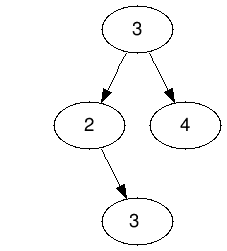
\includegraphics[width=0.3\columnwidth]{fig/bst_duplicate.png}
    \caption{A BST with nodes 3 duplicated twice.}
    \label{fig:bst_duplicate}
\end{figure}
Note that the duplicates are not in contiguous levels. This is a big issue when allowing duplicates in a BST representation as, because  duplicates may be separated by any number of levels, making the detection of duplicates difficult.

An option to avoid this issue is to not represent duplicates structurally (as separate nodes) but instead use a \texttt{counter} that counts the number of occurrences of the key. The previous example will be represented as in Fig.~\ref{fig:bst_duplicate_counter}:
\begin{figure}[H]
    \centering
    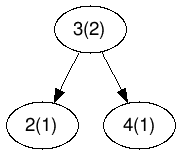
\includegraphics[width=0.3\columnwidth]{fig/bst_duplicate_counter.png}
    \caption{A BST with nodes 3 marked with two occurrence.}
    \label{fig:bst_duplicate_counter}
\end{figure}

This simplifies the related operations at the expense of some extra bytes and counter operations. Since a heap is a complete binary tree, it has a smallest possible height - a heap with N nodes always has O(log N) height. 



%%%%%%%%%%%%%%Segment Tree%%%%%%%%%%%%%%%
\section{Segment Tree}
\label{sec_segment_tree}
To answer queries over an array is called a \textit{range query problem}, e.g. finding the sum of consecutive subarray $a[l:r]$, or finding the minimum item in such a range. A direct and linear solution is to compute the required query on the subarray on the fly each time. When the array is large, and the update is frequent, even this linear approach will be too slow. Let's try to solve this problem faster than linear. How about computing the query for a range in advance and save it in a dictionary? If we can, the query time is constant. However, because there are $n^2$ subarray, making the space cost polynomial, which is definitely not good.  Another problem, ``what if we need to change the value of an item'', we have to update $n$ nodes in the dictionary which includes the node in its range. 

We can balance the search, update, and space from the dictionary approach to a logarithmic time with the technique of decrease and conquer. In the binary search, we keep dividing our search space into halves recursively until a search space can no longer be divided. We can apply the dividing process here, and construct a binary tree, and each node has \texttt{l} and \texttt{r} to indicate the range of that node represents. For example, if our array has index range $[0, 5]$,  its left subtree will be [0, mid], and right subtree will be [mid+1, 5]. a binary tree built with binary search manner is shown in Fig.~\ref{fig:segment_tree_range}.
\begin{figure}[H]
    \centering
    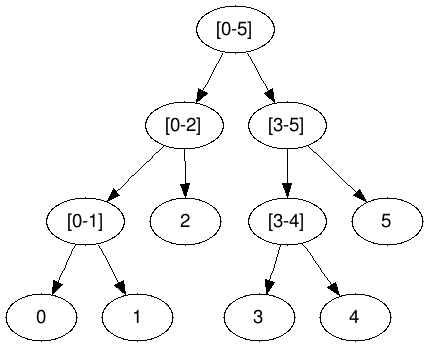
\includegraphics[width=0.6\columnwidth]{fig/segment_tree_range.png}
    \caption{A Segment Tree }
    \label{fig:segment_tree_range}
\end{figure}
To get the answer for range query $[0, 5]$, we just return the value at root node. If the range is $[0, 1]$, which is on the left side of the tree, we go to the left branch, and cutting half of the search space. For a range that happens to be between two nodes, such as $[1, 3]$, which needs node \texttt{[0, 1]} and \texttt{[2-5]}, we search [0, 1] in the left subtree and [2, 3] in the right subtree and combine them together. Any searching will be within $O(\log n)$, relating to the height of the tree. \textcolor{red}{needs better complexity analysis} 

\paragraph{Segment tree} The above binary tree is called \textbf{segment tree}. From our analysis, we can see a segment tree is a static full binary trees. 'Static` here means once the data structure is built, it can not be modified or extended.  However, it can still update the value in the original array into the segment tree. Segment tree is applied widely to efficiently answer numerous \textit{dynamic range queries} problems 
(in logarithmic time), such as finding minimum, maximum, sum, greatest common divisor, and least common denominator in array.


Consider an array $A$ of size $n$ and a corresponding segment tree $T$:
\begin{enumerate}
    \item The root of $T$ represents the whole array $A[0:n]$. 
    \item Each internal node in $T$ represents the interval of $A[i:j]$ where $0 < i < j <= n$. 
    \item Each leaf in $T$ represents a single element A[i], where $0 \leq i<n$. 
    \item If the parent node is in range [i, j], then we separate this range at the middle position $m = (i+j)//2$; the left child takes range $[i, m]$, and the right child take the interval of $[m+1, j]$.
\end{enumerate}

Because in each step of building the segment tree, the interval is divided into two halves, so the height of the segment tree will be $\log n$. And there will be totally $n$ leaves and $n-1$ number of internal nodes, which makes the total number of nodes in segment tree to be $2n-1$, which indicates a linear space cost. Except of an explicit tree can be used to implement segment tree, an implicit tree implemented with  array can be used too, similar to the case of heap data structure. 

\subsection{Implementation}
Implementation of a functional segment tree consists of three core operations: tree construction, range query, and value update, named as as \texttt{\_buildSegmentTree()}, \texttt{RangeQuery()}, and \texttt{update()}, respectively. We demonstrate the implementation with Range Sum Query (RSQ) problem, but we try to generalize the process so that the template can be easily reused to other range query problems. In our implementation, we use explicit tree data structure for both convenience and easier to understand. We define a general tree node data structure as:
\begin{lstlisting}[language=Python]
class TreeNode:
  def __init__(self, val, s, e):
    self.val = val
    self.s = s
    self.e = e
    self.left = None
    self.right = None
\end{lstlisting}

%\begin{examples}[resume]
\paragraph{Range Sum Query(L307, medium)} Given an integer array, find the sum of the elements between indices i and j, range $[i, j], i\leq j$. 
\begin{lstlisting}[numbers=none]
Example:

Given nums = [2, 9, 4, 5, 8, 7]

sumRange(0, 2) -> 15
update(1, 3)
sumRange(0, 2) -> 9
\end{lstlisting}

\paragraph{Tree Construction}
\begin{figure}[h]
    \centering
    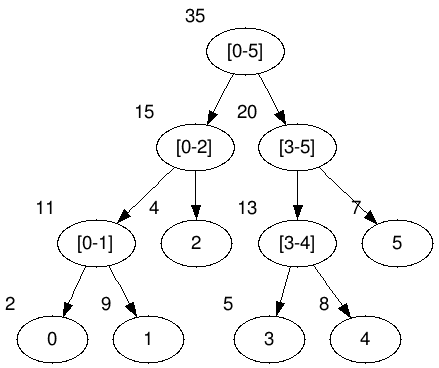
\includegraphics[width=0.6\columnwidth]{fig/segment_tree_construction.png}
    \caption{Illustration of Segment Tree for Sum Range Query. }
    \label{fig:segment_tree_construction}
\end{figure}
The function \texttt{\_buildSegmentTree()} takes three arguments: \texttt{nums}, \texttt{s} as the start index, and \texttt{e} as the end index. Because there are totally $2n-1$ nodes, which makes the time and space complexity both be $O(n)$.
\begin{lstlisting}[language=Python]
def _buildSegmentTree(nums, s, e):
  '''
   s, e: start index and end index
  '''
  if s > e:
      return None
  if s == e:
      return TreeNode(nums[s], s, e)
  
  m = (s + e)//2
  # Divide: return a subtree 
  left = _buildSegmentTree(nums, s, m)
  right = _buildSegmentTree(nums, m+1, e)
  
  # Conquer: merge two subtree
  node = TreeNode(left.val + right.val, s, e)
  node.left = left
  node.right = right
  return node
\end{lstlisting}
Building a segment tree for our example as:
\begin{lstlisting}[language=Python]
nums = [2, 9, 4, 5, 8, 7]
root = _buildSegmentTree(nums, 0, len(nums) - 1)
\end{lstlisting}
It will generate a tree shown in Fig.~\ref{fig:segment_tree_construction}. 
\paragraph{Range  Query}  Each query within range $[i, j], i < j, i\geq s, j \leq e$, will be found on a node or by combining multiple node. In the query process,  check the following cases:
\begin{itemize}
    \item 
    If range $[i, j]$ matches the range $[s, e]$, if it matches, return the value of the node, otherwise, processed to other cases.
    \item  Compute middle index $m = (s + e) // 2$. Check if range $[i, j]$ is within the left state space $[s, m]$ if $j\leq m$, or within the right state space $[m+1, e]$ if $i\geq m+1$, or is cross two spaces if otherwise. 
    \begin{itemize}
    \item For the first two cases, a recursive call on that branch will return our result.
    \item For the third case, where the range crosses two space, two recursive calls on both children of our current node are needed: the left one handles range $[i, m]$, and the right one handles range $[m+1, j]$. The final result will be a combination of these two. 
    \end{itemize}
\end{itemize}
The code is as follows: 
\begin{lstlisting}[language=Python]
def _rangeQuery(root, i, j, s, e): 
  if s == i and j == e:
    return root.val if root else 0 
  m = (s + e)//2
  if j <= m:
    return _rangeQuery(root.left, i, j, s, m)
  elif i > m:
    return _rangeQuery(root.right, i, j, m+1, e)
  else:
    return _rangeQuery(root.left, i, m, s, m) + _rangeQuery(root.right, m+1, j, m+1, e)
\end{lstlisting}
% The complete code is given: 
% \begin{lstlisting}[language=Python]
% class NumArray:
%     class TreeNode:
%         def __init__(self, val):
%             self.val = val
%             self.left = None
%             self.right = None

%     def __init__(self, nums):
%         self.n = 0
%         self.st = None
%         if nums:
%             self.n = len(nums)
%             self.st = self._buildSegmentTree(nums, 0, self.n-1)    
            
%     def update(self, i, val):
%         self._updateNode(i, val, self.st, 0, self.n -1)       

%     def sumRange(self, i, j):
%         return self._rangeQuery(self.st, i, j, 0, self.n-1)
% \end{lstlisting}
\paragraph{Update} To update \texttt{nums[1]=3}, all nodes on the path from root to the leaf node will be affected and needed to be updated with to incorporate the change at the leaf node. We search through the tree with a range $[1, 1]$ just like we did within \texttt{\_rangeQuery} except that we no longer need the case of crossing two ranges. Once we reach to the leaf node, we update that node's value to the new value, and it backtracks to its parents where we recompute the parent node's value according to the result of its children.   This operation takes $O(\log n)$ time complexity, and we can do it inplace since the structure of the tree is not changed. 
\begin{lstlisting}[language=Python]
def _update(root, s, e, i, val):
  if s == e == i:
    root.val = val
    return 
  m = (s + e) // 2
  if i <= m:
    _update(root.left, s, m, i, val)
  else:
    _update(root.right, m + 1, e, i, val)
  root.val = root.left.val + root.right.val
  return 
\end{lstlisting}

\paragraph{Minimum and Maximum Range Query} To get the minimum or maximum value within a given range, we just need to modify how to value is computed. For example, to update, we just need to change the line 10 of the above code to \texttt{root.val = min(root.left.val, root.right.val)}. 

There are way more other variants of segment tree, check it out if you are into knowing more at \url{https://cp-algorithms.com/data_structures/segment_tree.html}.

% \paragraph{Dynamic Programming for Static Array}




%%%%%%%%%%%%%%%%%%%%%%%%%Exercise%%%%%%%%%%%%%%%%%%%%%%%%%%%%%%%%%%%%%%%%%%%%%%%%
\section{Exercises}

\begin{enumerate}
    \item 144. Binary Tree Preorder Traversal
    \item 94. Binary Tree Inorder Traversal
    \item 145. Binary Tree Postorder Traversal
    \item 589. N-ary Tree Preorder Traversal
    \item 590. N-ary Tree Postorder Traversal
    \item 429. N-ary Tree Level Order Traversal
    \item 103. Binary Tree Zigzag Level Order Traversal(medium)
    \item 105. Construct Binary Tree from Preorder and Inorder Traversal
\end{enumerate}

938. Range Sum of BST (Medium)

Given the root node of a \textbf{binary search tree}, return the sum of values of all nodes with value between L and R (inclusive).

The binary search tree is guaranteed to have unique values.
\begin{lstlisting}
Example 1:

Input: root = [10,5,15,3,7,null,18], L = 7, R = 15
Output: 32

Example 2:

Input: root = [10,5,15,3,7,13,18,1,null,6], L = 6, R = 10
Output: 23
\end{lstlisting}
\textbf{Tree Traversal+Divide and Conquer}. We need at most $O(n)$ time complexity. For each node, there are three cases: 1) L <= val <= R, 2)val < L, 3)val > R. For the first case it needs to obtain results for both its subtrees and merge with its own val. For the others two, because of the property of BST, only the result of one subtree is needed. 
\begin{lstlisting}[language=Python]
def rangeSumBST(self, root, L, R):
    if not root:
        return 0
    if L <= root.val <= R:
        return self.rangeSumBST(root.left, L, R) + self.rangeSumBST(root.right, L, R) + root.val
    elif root.val < L: #left is not needed
        return self.rangeSumBST(root.right, L, R)
    else: # right subtree is not needed
        return self.rangeSumBST(root.left, L, R)
\end{lstlisting}

\subsection{Exercises}
\begin{examples}
\item \textbf{35. Search Insert Position (easy).} Given a sorted array and a target value, return the index if the target is found. If not, return the index where it would be if it were inserted in order.

You can assume that there are no duplicates in the array.
\begin{lstlisting}[numbers=none]
Example 1:

Input: [1,3,5,6], 5
Output: 2

Example 2:
Input: [1,3,5,6], 2
Output: 1

Example 3:
Input: [1,3,5,6], 7
Output: 4

Example 4:
Input: [1,3,5,6], 0
Output: 0
\end{lstlisting}

\textbf{Solution: Standard Binary Search Implementation.} For this problem, we just standardize the Python code of binary search, which takes $O(logn)$ time complexity and O(1) space complexity without using recursion function. In the following code, we use exclusive right index with len(nums), therefore it stops if l == r; it can be as small as 0 or as large as n of the array length for numbers that are either smaller or equal to the nums[0] or larger or equal to nums[-1]. We can also make the right index inclusive. 
\begin{lstlisting}[language = Python]
# exclusive version
def searchInsert(self, nums, target):
    l, r = 0, len(nums) #start from 0, end to the len (exclusive)
    while l < r:
        mid = (l+r)//2
        if nums[mid] < target: #move to the right side
            l = mid+1
        elif nums[mid] > target: #move to the left side, not mid-1
             r= mid
        else: #found the traget
            return mid
    #where the position should go
    return l
\end{lstlisting}

\begin{lstlisting}[language = Python]
# inclusive version
def searchInsert(self, nums, target):
   l = 0
    r = len(nums)-1
    while l <= r:
        m = (l+r)//2
        if target > nums[m]: #search the right half
            l = m+1
        elif target < nums[m]: # search for the left half
            r = m-1
        else:
            return m
    return l
\end{lstlisting}
\end{examples}
Standard binary search
\begin{enumerate}
    \item 611. Valid Triangle Number (medium)
    \item 704. Binary Search (easy)
    
\item  74. Search a 2D Matrix) Write an efficient algorithm that searches for a value in an m x n matrix. This matrix has the following properties:
\begin{enumerate}
    \item Integers in each row are sorted from left to right.
    \item The first integer of each row is greater than the last integer of the previous row.
    \end{enumerate}
\begin{lstlisting}[numbers=none]
For example,
Consider the following matrix:

[
  [1,   3,  5,  7],
  [10, 11, 16, 20],
  [23, 30, 34, 50]
]

Given target = 3, return true.
\end{lstlisting}

% Solution: 2D matrix search, time complexity from $O(n^2)$ to $O(lgm+lgn)$.
% \begin{lstlisting}[language = Python]
% def searchMatrix(self, matrix, target):
%         """
%         :type matrix: List[List[int]]
%         :type target: int
%         :rtype: bool
%         """
        
%         if not matrix:
%             return False
%         row, col = len(matrix), len(matrix[0])
%         if row==0 or col==0: #for [[]]
%             return False
%         sr, er = 0, row-1
%         #fisrst search the mid row
%         while sr<=er:
%             mid = sr+(er-sr)//2
%             if target>matrix[mid][-1]: #go to the right side
%                 sr=mid+1
%             elif target < matrix[mid][0]: #go the the left side
%                 er = mid-1
%             else: #value might be in this row
%                 #search in this row
%                 lc, rc = 0, col-1
%                 while lc<=rc:
%                     midc = lc+(rc-lc)//2
%                     if matrix[mid][midc]==target:
%                         return True
%                     elif target<matrix[mid][midc]: #go to left
%                         rc=midc-1
%                     else:
%                         lc=midc+1
%                 return False
%         return False
% \end{lstlisting}

Also, we can treat is as one dimensional, and the time complexity is $O(lg(m*n))$, which is the same as $O(log(m)+log(n))$.
\begin{lstlisting}[language = Python]
class Solution:
    def searchMatrix(self, matrix, target):
        if not matrix or target is None:
            return False

        rows, cols = len(matrix), len(matrix[0])
        low, high = 0, rows * cols - 1
        
        while low <= high:
            mid = (low + high) / 2
            num = matrix[mid / cols][mid % cols]

            if num == target:
                return True
            elif num < target:
                low = mid + 1
            else:
                high = mid - 1
        
        return False
\end{lstlisting}
\end{enumerate}

Check \url{http://www.cnblogs.com/grandyang/p/6854825.html} to get more examples.

Search on rotated and 2d matrix:
\begin{enumerate}
    \item 81. Search in Rotated Sorted Array II (medium) 
    \item 153. Find Minimum in Rotated Sorted Array (medium) The key here is to compare the mid with left side, if mid-1 has a larger value, then that is the minimum 
    \item 154. Find Minimum in Rotated Sorted Array II (hard)
\end{enumerate}
Search on Result Space:
\begin{enumerate}
    \item 367. Valid Perfect Square (easy) (standard search)
    \item 363. Max Sum of Rectangle No Larger Than K (hard)
    \item 354. Russian Doll Envelopes (hard)
    \item 69. Sqrt(x) (easy)
\end{enumerate}


% \subfile{chapters/chapter_9_linear_searching}
%  \subfile{chapters/chapter_13_tree_algorithm}
 \end{document}